%%%%%%%%%%%%%%%%%%%%%%%%%%%%%%%%
%% What is an event? 
%%%%%%%%%%%%%%%%%%%%%%%%%%%%%%%%

% add picture of CMS event display
% add picture of hadronization etc for event

At the LHC we define an \textit{event} as everything that happens in a proton bunch crossing.
These high energy collisions are very complex, often resulting in the production of many hundreds of
particles. An illustration of this complexity is shown in Fig.~\ref{fig:event_full_event}.
A proper escription of what happens is impeded by the composite nature of the proton, and by the
consequences of the strong coupling constant of QCD, the quantum field theory governing hadron
interactions.
Fortunately, it turns out that the full process can be factorized into independent subprocesses,
each taking place at different energy scales. 


\begin{figure}[htpb]
  \centering
  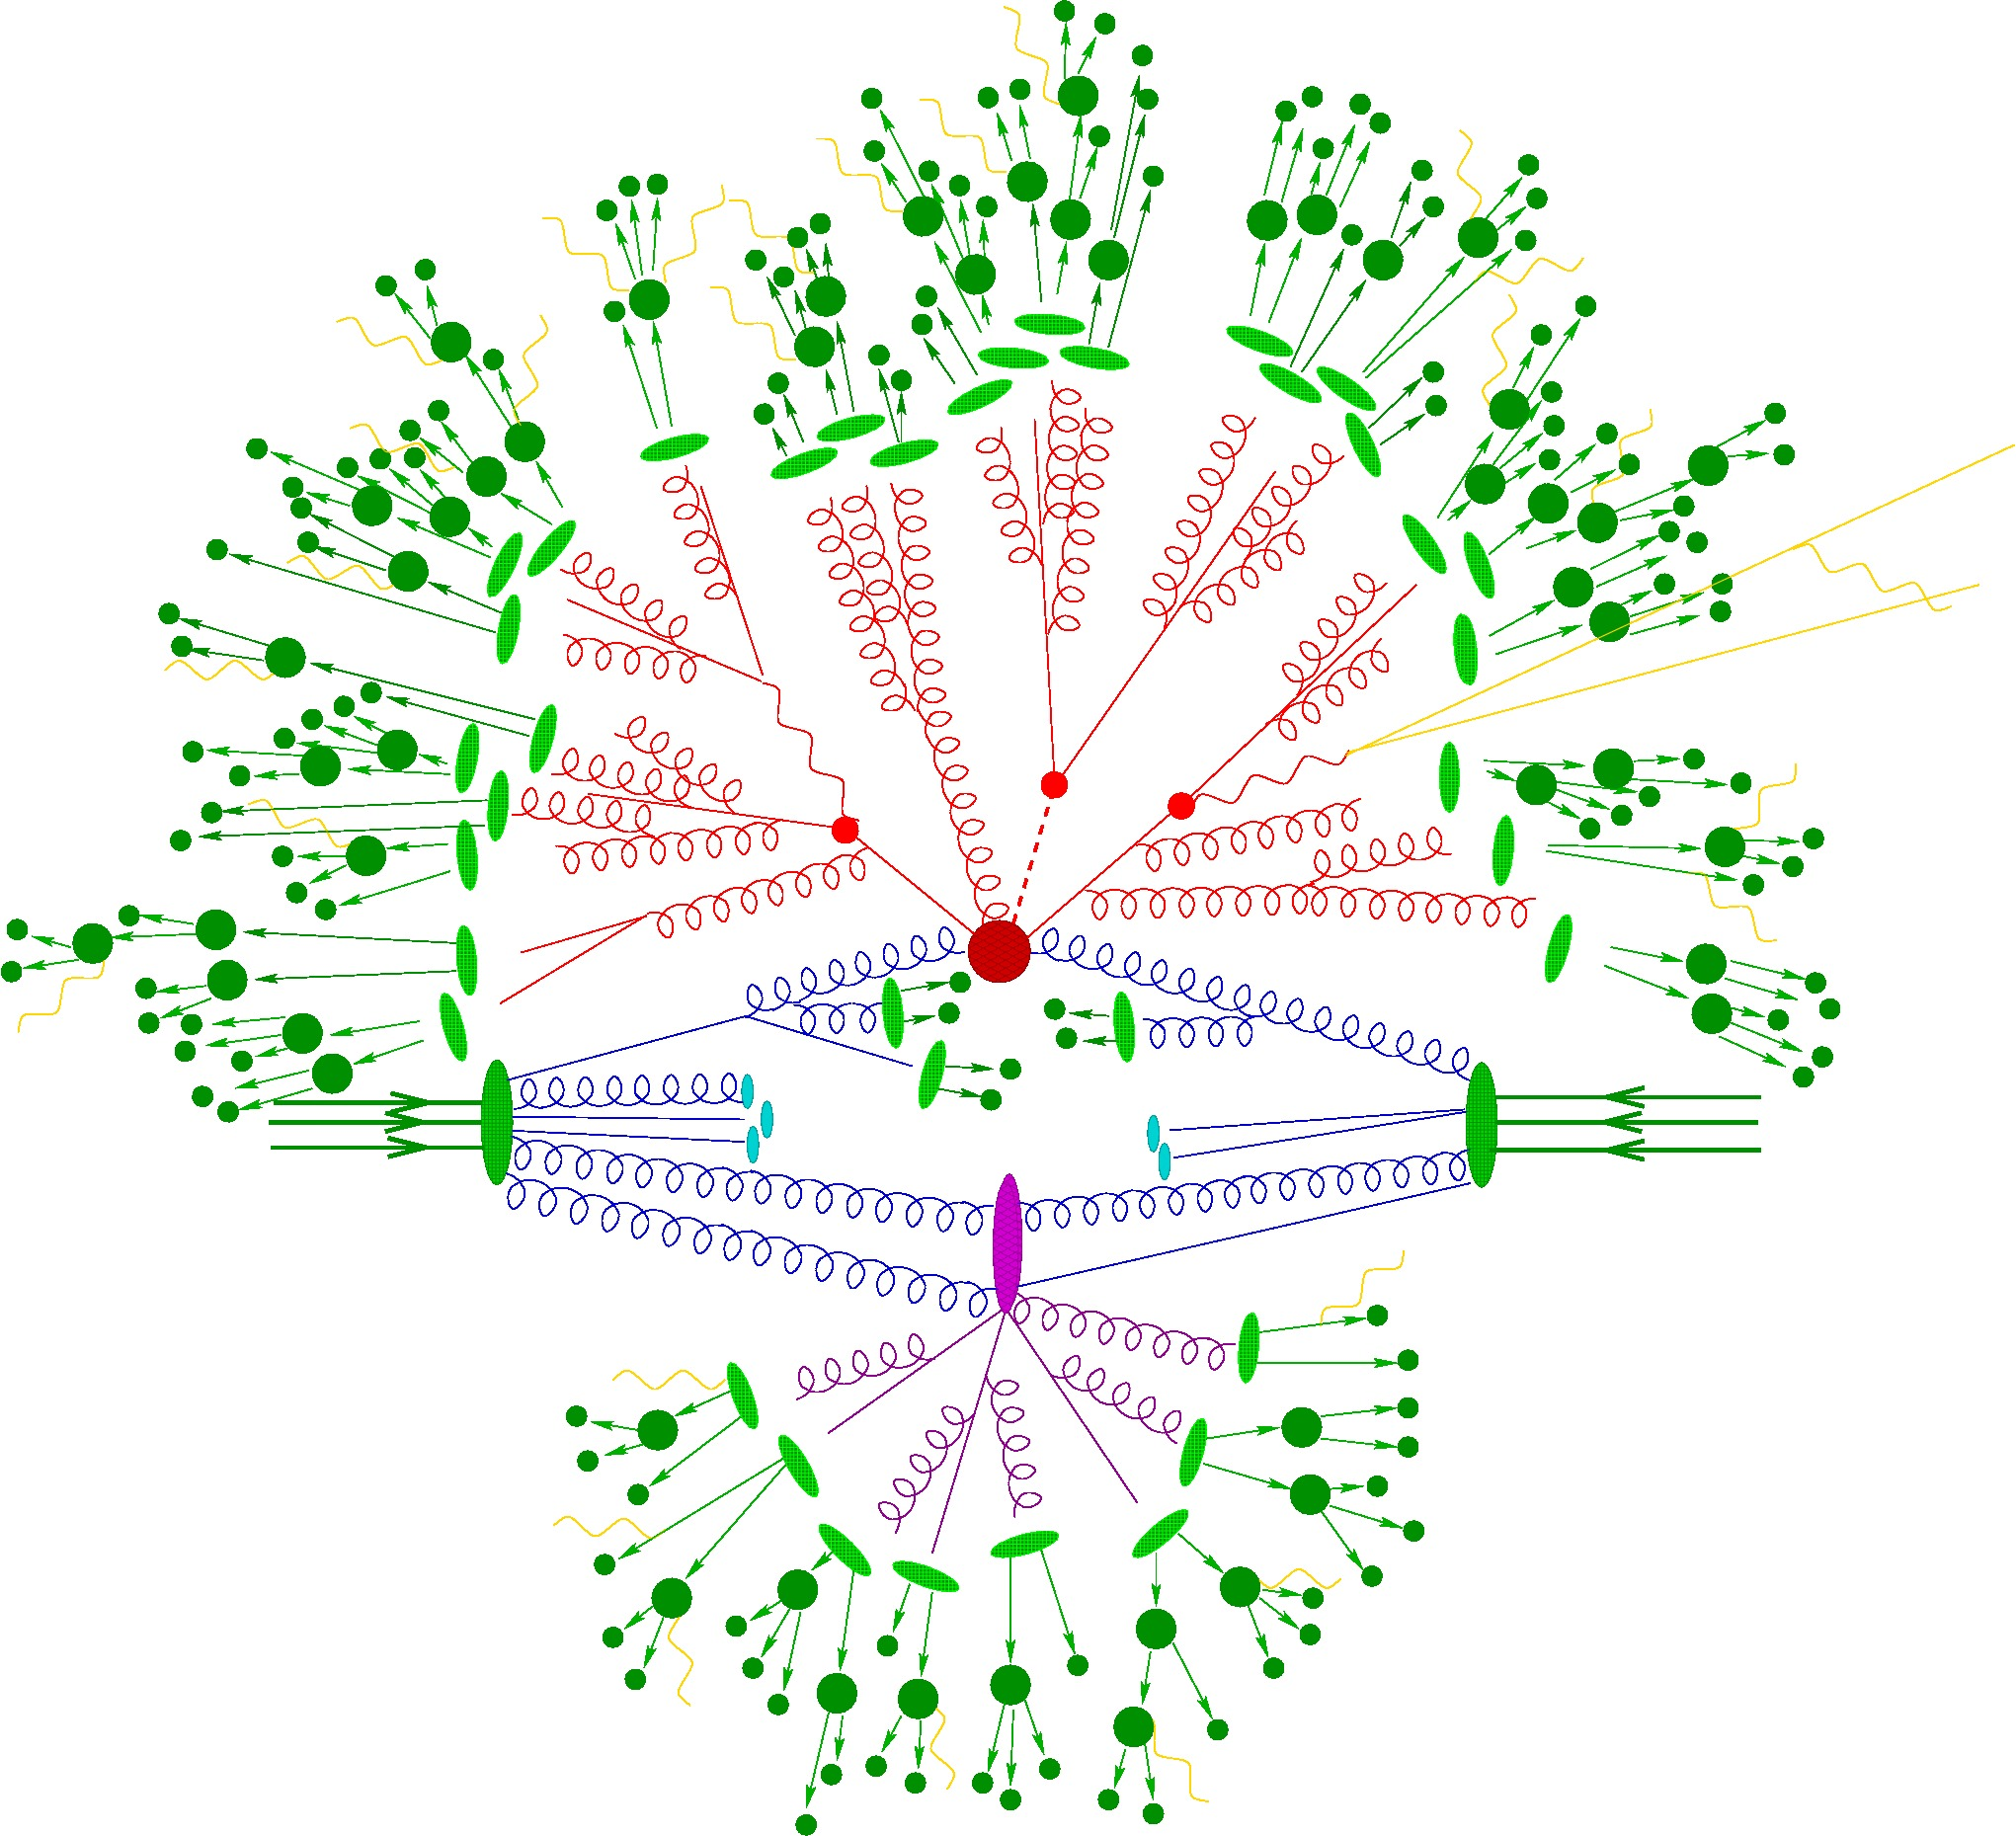
\includegraphics[width=0.8\textwidth]{figures/eventreco_event/full_event}
  \caption{Pictorial representation of a $\Pp\Pp$ collision event.
The hard interaction (big red blob) is followed by the decay of the produced particles (small red
blobs).
Additional hard QCD radiation is produced (red) and a secondary interaction takes place (purple
blob) before the final-state partons hadronize (light green blobs) and hadrons decay (dark green
blobs). Photon radiation occurs at any stage (yellow). Figure taken from
Ref.~\cite{Gleisberg:2008ta}
  \label{fig:event_full_event}}
\end{figure}


The process that is usually of most interest is the interaction between the constituents of the two
protons that results in high \pt particles. This is referred to as the \textit{hard interaction}. 
Not every collision produces very hard particles, sometimes protons mearly undergo elastic
collisions, resulting in very soft scattering products that do not pass the detection thresholds. In
general, any interaction producing some detectable particles is called a \textit{minimum bias
interaction}. 

The initial momentum distribution of the partons involved in the hard interaction is contained
within \textit{parton distribution functions} (PDFs) describing the structure of the proton. 
Apart from the hard interaction, the other constituents of the proton can also interact. This
usually results in a spray of softer particles, the \textit{underlying event} (UE). 
Any high momentum particle produced in the collision will emit additional hard QCD radiation, the
so-called initial- and final-state-radiation (ISR or FSR).

Quarks and gluons produced in the collision cannot stay free, they must hadronize in a time scale
of $\mathcal{O}(\text{10}^{\text{-23}}\second)$. These hadrons, in addition to possible produced
leptons, will then pass through the experiment where they can be detected, and used to find out
what happened in the collision itself. An example of how a collision might look like in the CMS
detector is shown in Fig.~\ref{fig:event_display}. 

In the next subsections I will elaborate on how to describe an event in a more mathematical way,
starting from the factorization theorem.

\begin{figure}[htpb]
  \centering
  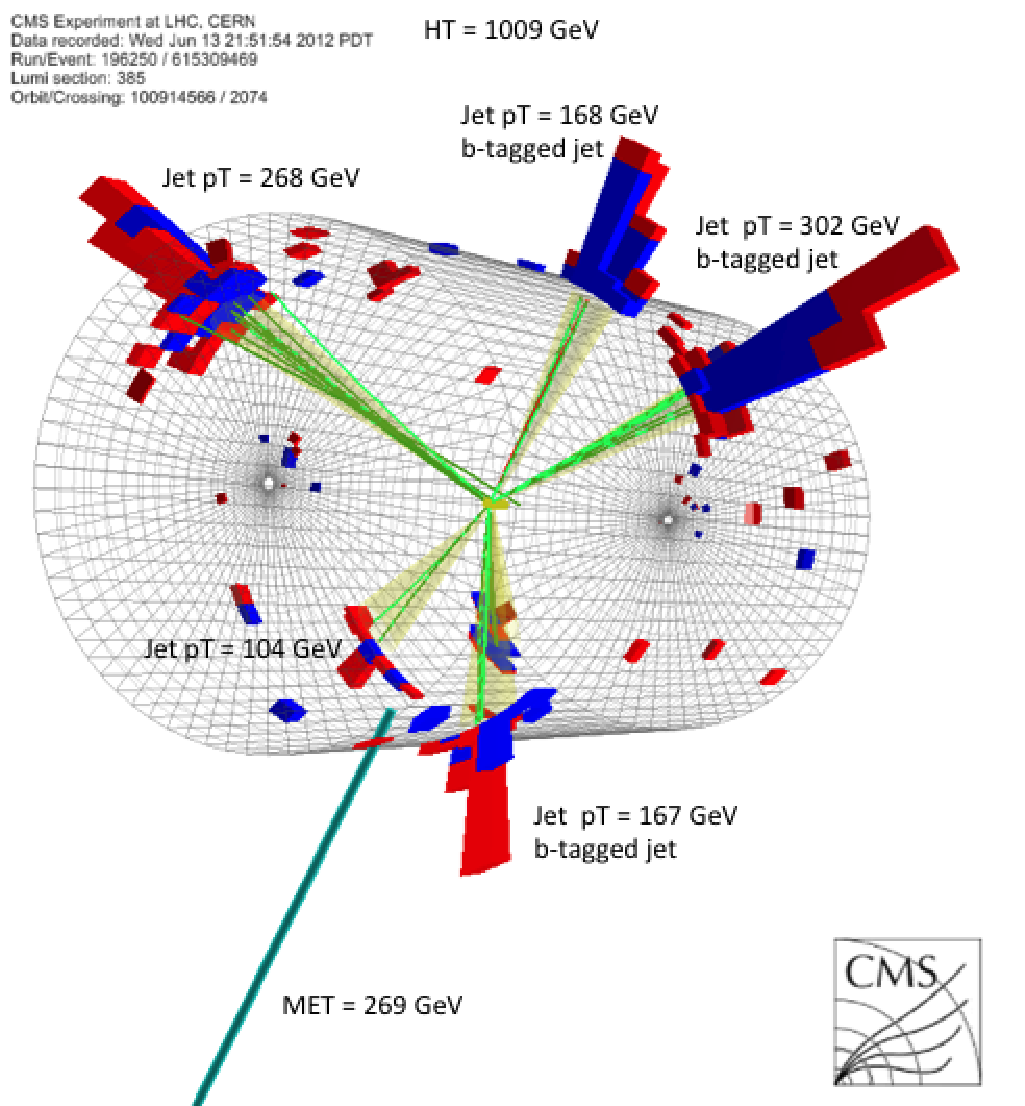
\includegraphics[width=0.7\textwidth]{figures/eventreco_event/event_display_SUS12024}
  \caption{CMS event display showing five high \pt jets, three of which are tagged as coming from a
$\cPqb$ quark. Figure from~\cite{SUS12024_event_display}.
  \label{fig:event_display}}
\end{figure}


\subsection{Factorization theorem}

\subsection{Parton distribution function}

\subsection{Hard interaction}

% mention following things: 
% - perturbation theory applies
% - complications arising from MPI
% - make link to section on matrix element generators which will contain more info on the practical
% implementation
